\chapter{Methods}

\section{COMSOL}
\label{sec:section11}
All resonator geometries were modelled and solved using COMSOL Multiphysics®
6.0, a finite element analysis (FEA) software package designed for the
simulation of complex physical systems. COMSOL uses edge element discretisation,
which is well suited to solving Maxwell’s equations for electromagnetic wave
propagation. This technique preserves the continuity of tangential electric
field components across element boundaries, which is particularly important in
high-frequency dielectric structures such as MASER resonators.

Due to the rotational symmetry of the resonator designs used in this project,
all simulations were carried out using COMSOL’s ‘axisymmetric 2D mode’. This
mode assumes azimuthal symmetry about the central axis and enables the reduction
of a 3D problem to a 2D cross-section, significantly reducing computational time
and memory requirements without sacrificing physical accuracy. In this
simplified geometry, the dielectric resonator is modelled as a rectangular
domain embedded in a rectangular air-filled cavity with metallic boundaries.

Each model comprised a dielectric resonator with a parametrised geometry and a
surrounding air domain enclosed by a metal cavity. Copper was selected as the
cavity material and modelled using an Impedance Boundary Condition to account
for realistic surface losses. The surrounding air domain was included to prevent
boundary reflections and to represent free-space propagation conditions. All
materials were assigned appropriate electromagnetic properties, including
relative permittivity, electric conductivity and relative permeability values.
The gain medium was also approximated to have a relative permittivity equal to
that of air, so it can simply be modelled as an air domain.

The initial dimensions of the resonator geometry were taken from the design
reported in the “MASER-in-a-Shoebox” study by Ng et al.\autocite{ng2023maser},
Table \ref{fig:table1}. They demonstrated a compact, room-temperature,
zero-field MASER. These baseline dimensions provided a realistic starting point
for frequency scaling and optimisation. To facilitate flexible geometry control
within COMSOL and ease integration with the optimisation process, the resonator
model was constructed using piecewise regular domains. This approach allowed
independent manipulation of features such as dielectric radius and the relative
permittivity values, enabling efficient parameter updates.

\begin{figure}[htbp]
  \centering
  \begin{minipage}{0.65\textwidth}
    \centering
    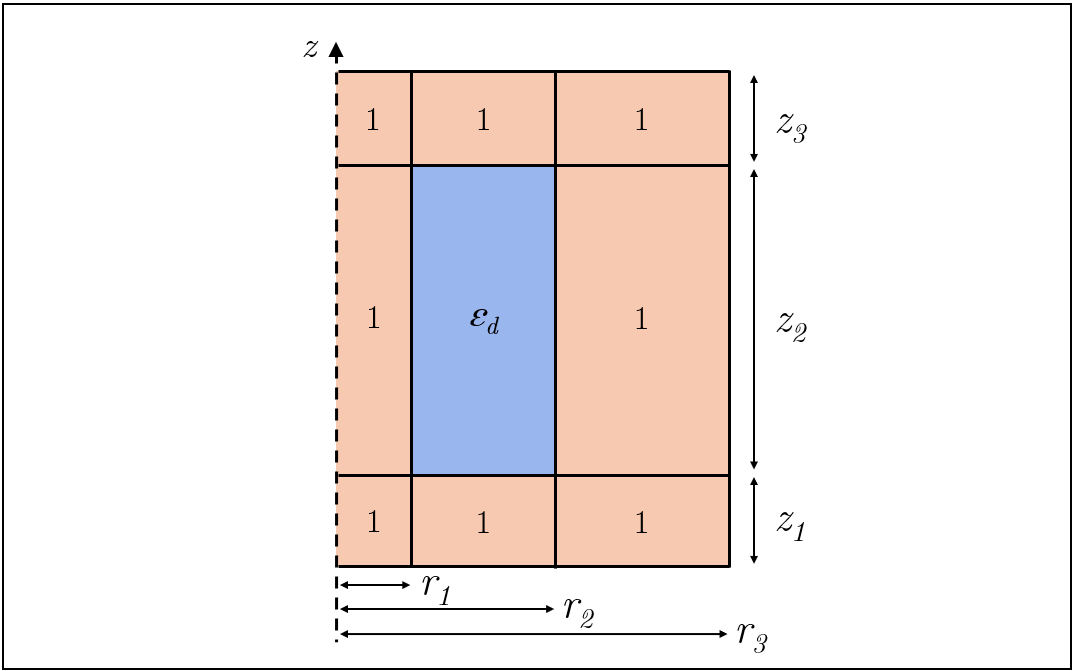
\includegraphics[width=\textwidth]{figures/figure8.png}
    \caption{
      Schematic of the 2D axisymmetric model geometry used in simulations. The
      structure is divided into subdomains with defined radial $(r_1,r_2,r_3)$
      and vertical $(z_1,z_2,z_3)$ dimensions. Each subdomain is assigned a
      relative permittivity, with air regions set to 1 and the dielectric core
      set to $\varepsilon_d$. This layout enables controlled manipulation of
      material boundaries and electromagnetic field confinement within the
      simulation domain.
    }
    \label{fig:figure8}
    \end{minipage}
  \hfill
  \begin{minipage}{0.31\textwidth}
    \centering
    \captionof{table}{
      The input parameters of the baseline model, based off of the dimensions of
      the MASER-in-a-Shoebox\autocite{ng2023maser}
    }
    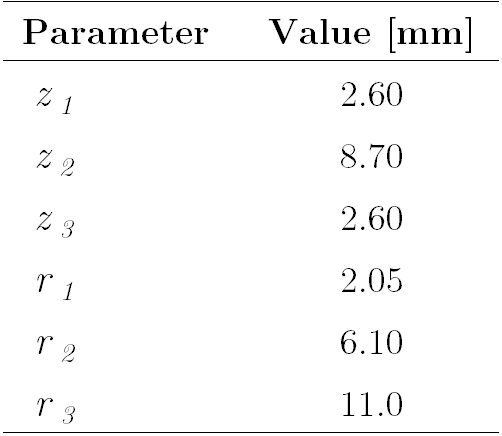
\includegraphics[width=\textwidth]{tables/table1.png}
    \label{fig:table1}
    \end{minipage}
\end{figure}

To ensure model fidelity, the published dimensions from the MASER-in-a-Shoebox
study were first replicated in COMSOL to serve as a geometric baseline. However,
the original structure did not resonate precisely at the target frequency of
1.45 GHz. To correct this, small adjustments were made to the vertical
dimensions $z_1$ and $z_3$, effectively mimicking the practical tuning mechanism
of a physical MASER resonator (like adjusting the cavity ceiling) to align the
resonance with the desired frequency. After tuning, the model was confirmed to
support the $\text{TE}_{01\delta}$ mode with strong magnetic field confinement
in the dielectric region. This verified geometry was then used as a benchmark
for evaluating all optimised configurations. Qualitative inspection of the field
distributions also ensured that optimised geometries consistently exhibited the
correct mode and avoided convergence onto non-masing solutions.

To enable control over the resonator’s shape during optimisation, a
$10\times 10$ rectangular subgrid was defined over the domain that contains the
dielectric resonator. Each element of this subgrid represents a small region
whose material properties can be independently adjusted. This complex structure
would be time consuming to produce manually in COMSOL, so I wrote a code
executable in COMSOL’s Application Builder to automate this process (can be
found in Appendix \ref{Appendix2}).

By assigning either the relative permittivity of the dielectric material (see
$\varepsilon_r$ column in Table \ref{table4}) or that of air
($\varepsilon_r$=1), each region can be treated as a binary switch, effectively
functioning like a binary matrix embedded within the continuous geometry. This
approach allows the overall shape of the resonator to be modified
programmatically by toggling the permittivity in individual regions, enabling
the genetic algorithm to explore a large variety of pixelated or composite
geometries without redefining the full domain or rebuilding the mesh manually.

\begin{figure}[htbp]
  \centering
  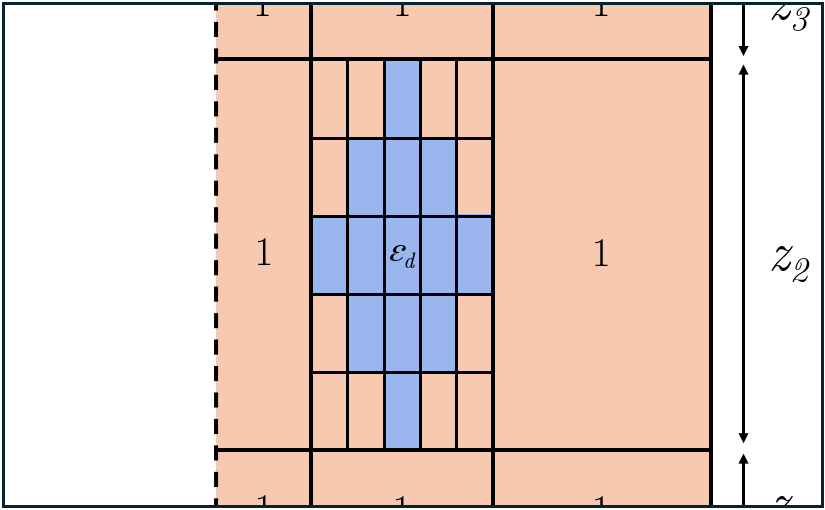
\includegraphics[width=0.7\textwidth]{figures/figure9.png}
  \caption{
    Illustration of the $N\times N$ subgrid method used to define dielectric
    geometry within the resonator. Each square element in the grid can be
    toggled between air ($\varepsilon_r=1$) and dielectric
    ($\varepsilon_r=\varepsilon_d$) to form arbitrary shapes. In this example, a
    $5\times 5$ grid is used to generate a central star-like structure embedded
    within the air-filled region.
  }
  \label{fig:figure9}
\end{figure}

The primary goal of each simulation was to evaluate the magnetic field
distribution $\vec{\mathbf{H}}$ and the electric field distribution
$\vec{\mathbf{E}}$, from which the quality factor, $Q_F$, and mode volume,
$V_m$, could be computed. Then therefore being able to calculate
$\frac{Q_f}{V_m}$ which is proportional to $F_P$ (the optimisation metric), as
seen in Equation \ref{Purcell}.

All models were meshed using extremely coarse triangular elements. This was to
reduce simulation time as much as possible as many concurrent simulations were
to be run during the genetic algorithm. Mesh settings were kept consistent
across all simulations to avoid introducing artificial variance in the computed
electromagnetic quantities. Not having to repeatedly remesh each model also cut
computational cost significantly, Because of the axisymmetric assumption, this
2D approach allowed for rapid evaluation of hundreds of resonator
configurations, making it well suited to integration with the genetic algorithm
discussed in the next section.

As with all finite element simulations, the results are subject to
discretisation errors. The use of an extremely coarse mesh reduced computation
time but may introduce systematic underestimation of the quality factor and
slight distortion of field distributions. However, because all geometries were
compared under identical meshing conditions, relative performance trends are
expected to remain valid. In addition, uncertainties in material parameters,
particularly the dielectric loss tangent and permittivity at GHz frequencies,
introduce some variability in Purcell factor estimation.

Finally, each COMSOL model was exported as a \texttt{.java} file.

\section{Java (COMSOL API) – Genetic Algorithm}
\label{sec:section12}
The primary objective of this project was to find the optimal shape and size of
a dielectric resonator that maximises the Purcell factor. To efficiently search
the large and discrete design space of possible resonator geometries, a Genetic
Algorithm (GA) was implemented and integrated directly with the COMSOL model via
the COMSOL Java API. This allowed for automated, iterative variation of the
resonator structure based on performance feedback from electromagnetic
simulations.

The .java file was then opened using Eclipse IDE (Integrated Development
Environment). Eclipse IDE was used for its extensible plug-in system for
customising the environment. The COMSOL plug-ins can be referenced within
Eclipse IDE in order to run COMSOL simulations without opening the COMSOL GUI
(Graphical User Interface).

The GA I wrote in Java (Appendix \ref{Appendix3}) using the Jenetics
library\autocite{wilhelmsen_jenetics}, can be appended to the .java file and
executed. Each candidate solution (i.e. resonator shape) was represented as a
100-bit binary chromosome, corresponding to a 10×10 subgrid over the resonator
region. In this representation, each bit determines whether a corresponding
domain is filled with the dielectric material (bit = 0) or replaced with air
(bit = 1). This effectively enabled the GA to act on a binary material matrix,
where the geometry could be adjusted by toggling local permittivity values
within a fixed simulation domain.

Before running the full optimisation, the genetic algorithm required an
initialised model that was structurally compatible with the 10×10 binary
chromosome format. To generate this, a 50/50 configuration was created by
applying a checkerboard-like pattern of dielectric and air-filled domains over
the resonator region of the baseline model (Figure \ref{fig:figure10}). This
approach ensured that the starting geometry reflected an unbiased, intermediate
state between fully filled and fully empty configurations—common practice in GA
initialisation to promote exploratory diversity in early generations. Because
this modified structure altered the effective dielectric loading of the cavity,
its permittivity was then iteratively scaled so that it resonated at the target
frequency of 1.45 GHz. This frequency alignment ensured that the GA started from
a physically valid configuration and that all subsequent fitness comparisons
were made relative to a consistent operating point. Now the GA could be run.

\begin{figure}[htbp]
  \centering
  \begin{minipage}{0.65\textwidth}
    \centering
    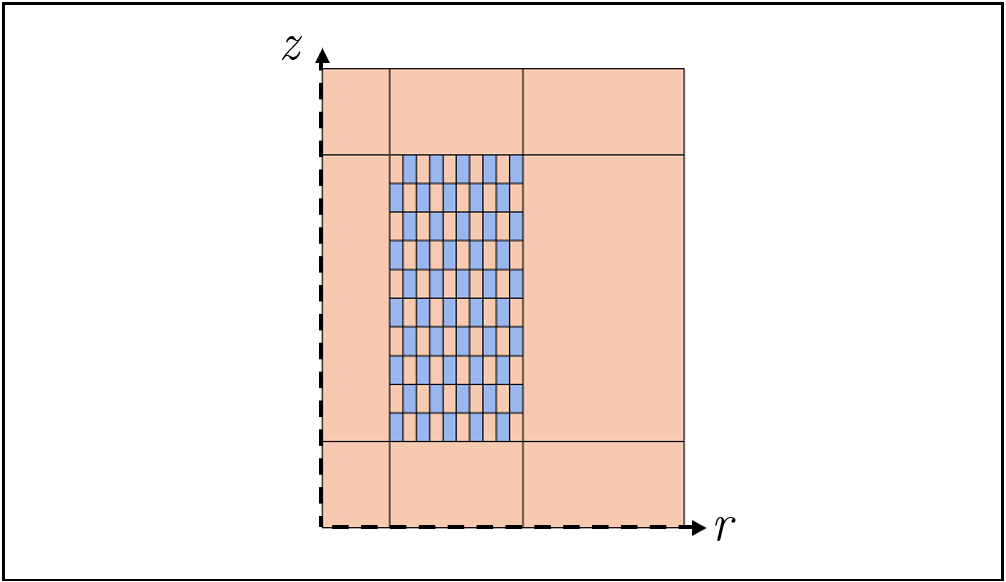
\includegraphics[width=\textwidth]{figures/figure10.png}
    \caption{
      Initialised configuration of the dielectric subgrid before the genetic
      algorithm is run. A checkerboard-like $10\times 10$ binary pattern is
      applied within the resonator region, alternating between air and
      dielectric elements. This balanced configuration promotes genetic
      diversity and serves as an unbiased starting point for optimisation.
    }
    \label{fig:figure10}
    \end{minipage}
  \hfill
  \begin{minipage}{0.31\textwidth}
    \centering
    \captionof{table}{The input parameters of the initialised model.}
    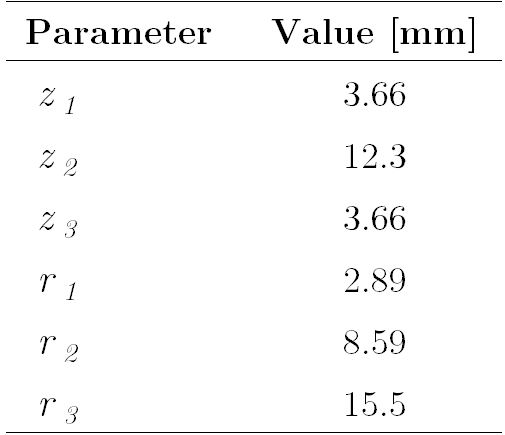
\includegraphics[width=\textwidth]{tables/table2.png}
    \label{fig:table2}
    \end{minipage}
\end{figure}

In each generation, the GA evaluated a population of 20 geometries over 250
generations. Standard evolutionary operators were used, including mutation
(5\%), crossover (80\%), and tournament selection also with elite selection.
Mutation introduces small, random changes to a geometry’s binary matrix,
flipping a few dielectric/air regions, to maintain diversity in the population
and avoid premature convergence. Crossover involves combining parts of two
parent dielectric geometries (binary matrices) to create new offspring
geometries, potentially inheriting favourable features from each parent.
Together, these operations allow the genetic algorithm to explore a wide design
space and progressively evolve higher-performing resonator shapes. Tournament
selection describes when two random subsets of a population of 2-5 geometries
are created and the individuals with the highest ‘fitness’ will have 80\% chance
that they will crossover. Elite selection automatically ensures that the
geometries with the highest ‘fitness’ carry over into the next generation. An
overview of the GA is shown in Figure \ref{fig:figure21}.

\begin{figure}[htbp]
  \centering
  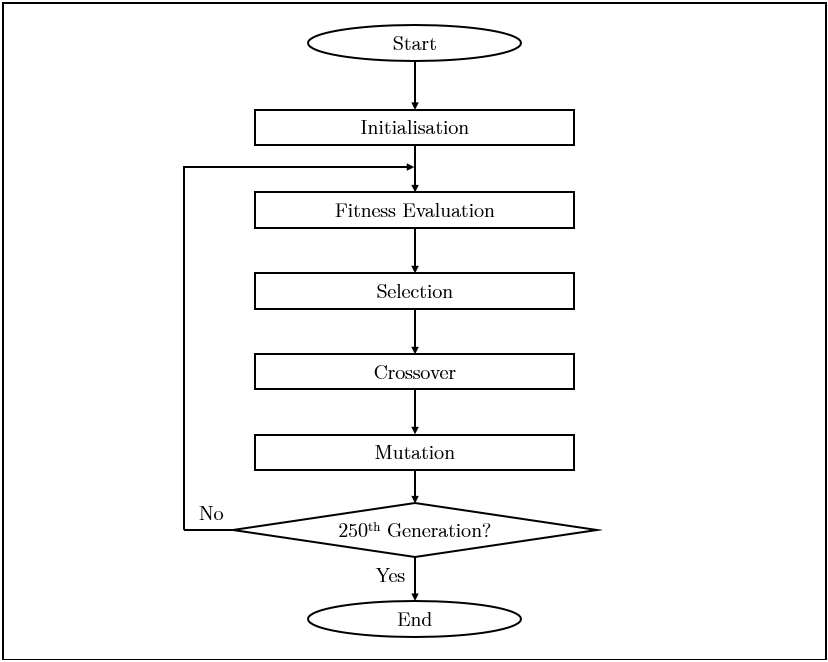
\includegraphics[width=0.6\textwidth]{figures/figure21.png}
  \caption{
    Flowchart illustrating the genetic algorithm (GA) process used for the
    optimisation of STO dielectric resonators. The algorithm begins with
    population initialization, followed by iterative cycles of fitness
    evaluation, selection, crossover, and mutation. The loop continues until the
    250th generation is reached, at which point the algorithm terminates. This
    structure allows for evolutionary exploration of geometries to improve
    $Q_f/V_m$.
  }
  \label{fig:figure21}
\end{figure}

Fitness was assigned based on the calculated Purcell factor (higher the $F_P$
the higher the fitness), which was extracted from each COMSOL run. The
simulation results computed the frequency, quality factor, and magnetic flux
density, hence $V_m$ can be calculated(see Equation \ref{eq:mode_volume}).

To ensure the resonator operated near the target MASER frequency of 1.45 GHz,
the GA included an adaptive permittivity scaling loop within each fitness
evaluation. This loop aimed to compensate for frequency shifts introduced by
changes in geometry by adjusting the global dielectric permittivity, effectively
'retuning' each configuration without altering the physical dimensions and
therefore remeshing the model.

A frequency shift was first achieved by applying a scalar multiplier $\alpha$ to
the real part of the dielectric permittivity $\varepsilon_r$, such that:

\begin{equation}
  \varepsilon_{\text{scaled}} = \alpha~\varepsilon_r
\end{equation}

Since the resonant frequency, $f$, of a dielectric-loaded cavity is
approximately inversely proportional to the square root of the relative
permittivity:

\begin{equation}
  f \propto \frac{1}{\sqrt{\varepsilon_r}}
\end{equation}

The scaling factor required to move from an initial frequency, $f_0$
, to the target frequency $f_t = 1.45$ GHz is given by:
\begin{equation}
\alpha = \left( \frac{f_0}{f_t} \right)^2
\end{equation}

This allowed the GA to adjust $\varepsilon_r$ automatically and bring the
resonant frequency of each geometry closer to the desired value, ideally within
a $\pm10$ MHz tolerance. However, in practice, this method encountered issues
when implemented. When the scaling factor was applied, the target frequency was
rarely achieved. The algorithm would alternate between frequencies too high and
too low without the values getting any closer to the target frequency. The cause
of this is unknown, this method may be an oversimplification of the relationship
between $\varepsilon_r$ and $f$ in COMSOL.

To overcome this issue, a Lagrange interpolation method was implemented to
estimate the appropriate permittivity scaling that would result in resonance at
1.45 GHz. For three previously simulated data points
$(\varepsilon_1, f_1),\ (\varepsilon_2, f_2),\ (\varepsilon_3, f_3)$, the
Lagrange polynomial was constructed as:

\begin{equation}
  f(\varepsilon) =
    f_1 \cdot
    \frac{(\varepsilon - \varepsilon_2)(\varepsilon - \varepsilon_3)}
         {(\varepsilon_1 - \varepsilon_2)(\varepsilon_1 - \varepsilon_3)}
    + f_2 \cdot
    \frac{(\varepsilon - \varepsilon_1)(\varepsilon - \varepsilon_3)}
         {(\varepsilon_2 - \varepsilon_1)(\varepsilon_2 - \varepsilon_3)}
    + f_3 \cdot
    \frac{(\varepsilon - \varepsilon_1)(\varepsilon - \varepsilon_2)}
         {(\varepsilon_3 - \varepsilon_1)(\varepsilon_3 - \varepsilon_2)}
\end{equation}

This polynomial was inverted numerically to estimate the value of $\varepsilon$
that would produce $f(\varepsilon)=1.45$ GHz. This method allowed robust
frequency correction without the drawbacks of direct permittivity scaling,
enabling consistent evaluation of the fitness function across a diverse set of
resonator geometries.

Throughout the evolutionary process, data including the Purcell factor, scaling
factor $\alpha$, and material assignments were logged to \texttt{.csv} files for
later analysis. The final output of the algorithm was the dielectric geometry
that produced the highest Purcell factor, along with its associated field
distribution and frequency characteristics. This approach enabled the discovery
of non-obvious geometries with superior field confinement and loss minimisation,
effectively bypassing the limitations of manual or purely intuitive design.

Each COMSOL simulation ran in approximately 5 seconds using my personal machine
(Intel i7, 16.0 GB RAM). The full GA process, encompassing 250 generations and
20 individuals per generation, took approximately 8 hours of continuous
computation.

The final optimised model returned from the genetic algorithm needs to be scaled
to return the permittivity values back to the initial values in order for proper
comparison with the baseline model.

\section{Julia – Quantum Cumulants}
\label{sec:section13}
To evaluate masing performance, the optimised resonator configurations were
simulated using \texttt{QuantumCumulants.jl}, a Julia package for modelling open
quantum systems. The Julia code was adapted with permission from Xipeng Shu, and
can be found in Appendix \ref{Appendix4}. The system consisted of a microwave
cavity (Fock space) coupled to ten clusters of pentacene molecules, each treated
as a five-level spin system using the ClusterSpace abstraction. The system
Hamiltonian described coherent spin–photon interactions between the cavity field
and molecular transitions (notably between levels 3 and 5), while Lindblad
operators captured spontaneous emission, intersystem crossing, spin relaxation,
and cavity photon decay. Critically, parameters from the COMSOL simulations, the
quality factor $Q_f$ and mode volume $V_m$, were used to derive the photon decay
rate $\kappa$ and coupling strength g53 in the Julia model. The decay rate was
estimated as:

\begin{equation}
  \kappa = \frac{\omega_m}{Q_f}
  \label{eq:kappa}
\end{equation}

where $\kappa$ is the cavity decay rate. The coupling strength $g_{53}$ was
inferred from $V_m$, which links the cavity-enhanced emission rate to the local
field density (see Equation \ref{eq:coupling_rate}):

\begin{equation}
  g_{53} \propto \sqrt{\frac{1}{V_m}}
  \label{eq:g53}
\end{equation}

This scaling allowed consistent integration of the electromagnetic properties
from COMSOL into the quantum dynamics of the spin ensemble.
The system was simulated in two phases: optical pumping (0–200 $\mu$s) and free
evolution (200–500 $\mu$s). The time-dependent intracavity photon number
⟨$\langle a^\dagger a \rangle$⟩ was extracted and converted into MASER output
power via:

\begin{equation}
  P_{\text{out}}(t) = \hbar \omega_m \kappa \langle a^\dagger a \rangle (t)
  \label{Pout}
\end{equation}

Output power was plotted over time to verify masing behaviour. This model
provided a bridge between dielectric design and macroscopic maser performance
under realistic room-temperature conditions.
